\documentclass[a4paper,12 pt]{article}
\usepackage{color}
\usepackage{graphicx}
\usepackage[bahasa]{babel}

\title{{Rangkuman}}
\author{Basis Data}
\date{9/03/20}

\begin{document}
\maketitle

\begin{center}

\includegraphics[width=6cm]{poltekpos}
\end{center}

\begin{center}
\author{Disusun Oleh :}
\end{center}
\begin{center}
\author{Nama : M. Ilyas Tri Khaqiqi}
\end{center}
\begin{center}
\author{Npm : 1194050}
\end{center}
\begin{center}
\author{Kelas : D4 TI 1B}
\end{center}
\vspace{1cm}
\begin{center}
\textbf{Program Diploma IV Teknik Informatika}
\end{center}
\begin{center}
\textbf{Politeknik Pos Indonesia}
\end{center}
\begin{center}
\textbf{Bandung}
\end{center}
\begin{center}
\textbf{2020}
\end{center}




\newpage
\section{Basis Data}
\section{Basis Data}
\subsection{Pengertian}
	basis data ialah tempat atau gudang yang diperuntukkan untuk menampung informasi,nilai/value untuk mempresentasikan suatu kejadian atau berupa objek yang merupakan suatu bukti fakta. dan data yang telah diperoleh tersebut dijadikan suatu referensi untuk mengatasi berbagai masalah.
	
\subsection{Basis Data Berdasarkan Teori}
basis data ialah kumpulan himpunan data berupa banyak arsip yang menghubungan antara satu dengan yang lainnya dan di dalam nya tidak terdapat suatu redudansi(pengulangan). dengan tempat penyimpanan cengan media elektronis dan di olah sedemikian rupa untuk kedepannya bisa memberikan manfaat dan kemudahan dalam menghadapi suatu persoalan.
	
\subsection{Kunci Pada Basis Data}.

			Primay Key, adalah suatu kunci yang uniq dan menjadi ciri khas suatu data agar menjadi suatu pembeda dari suatu tabel. kunci tersebut adalah termasuk ciri agar tidak terjadi suatu redudansi. dan primary key itu ada yang terlihat dan ada juga yang tidak terlihat.
	
	Foreign Key, adalah suatu kunci tamu yang relasi dari suatu domainnya. jadi di saat primary key bertamu ke tabel lain sang primary key itu dalam kunjungannya berubah menjadi suatu foreign key.
	
	Candidate Key adalah suatu candidat yang bisa di jadikan suatu Prinary Key.
\subsection{Pangkat suatu basis data}
pangkat atau kedudukan suatu basis data itu yaitu dari satu ke satu, satu ke banyak, banyak ke satu, dan banyak ke banyak.

\newpage
\subsection{apa itu tabel master?}
apasih tabel master? tabel master itu adalah suatu tabel yang mempunyai keunggulan dapat mengambil informasi dari tabel yang saling berelasi dengannya

\subsection{Tujuan Basis Data}
tujuan dari suatu basis data ini ialah Speed, space, and acuracy. speed adalah suatu kecepatan dalam penyimpanan data dan kecepatan mengambil datanya juga.
space adalah suatu kemudahan untuk tempat penyimpana data yang besar tanpa membutuhkan ruangan yang besar.
acuracy ini adalah suatu kegesitan yang di berikan suatu basis data yang berdasarkan fakta yang akurat.

\subsection{Model Basis Data}
model yang terdapat di Basis Data Ini adalah Jaringan, Hirarki, Relasional. nah yang Relational itu memiliki suatu kemudahan dan dapat dengan mudah menghindari suatu redudansi dan sedangkan Jaringan dan Hirarki adalah kebalikan dari relational.
\subsection{tambahan yang harus Di dipahami}
word dan excel bukan aplikasi bagian dari basis data. karena dua aplikasi itu melanggar suatu aturan basis data yaitu menghindari perulangan. sedangkan di dalam dua aplikasi tersebut terus melakukan perulangan kata secara terus menerus

\subsection{Concep Data Model dan Physical Data Model}
\begin{center}
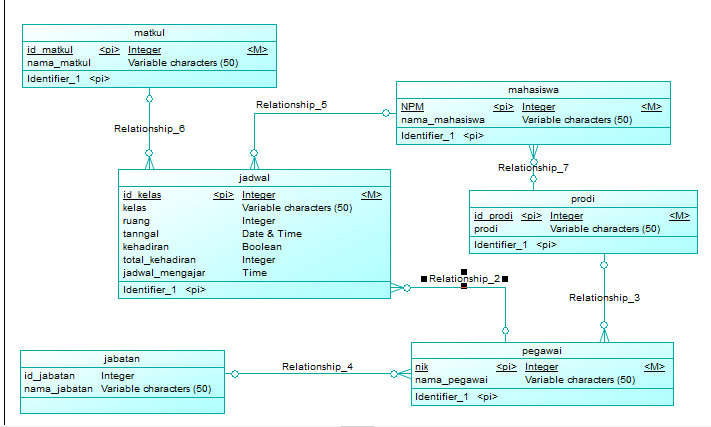
\includegraphics[width=10cm]{CDM}
\end{center}
sebelumnya untuk membentuk suatu data setelah kamu mengumpulkan data maka langkah selanjutnya juga oleh kamu uraikan dan siapa sih yang cocok saling berelasi. sebelum kamu membuat suatu rancangan seperti ini kamu harus melakukan suatu pengumpulan data terlebih dahulu, lalu menganalisa mana saja yang bisa di jadikan satu tabel. dan yang terakhir adalah merancangnya dari hasil pengumpulan nilai dan data tersebut. dan di hubungkan saling berelasi agar satu dengan yang lainnya mempunyai suatu kesatuan dalam menjalankannya. 
dan di atas adalah suatu gambar CDM yang mempunyai arti Concep Data Model jadi hanya suatu perealisasian dan belum nampak bagaimana arah suatu relasinya dan belum sepenuhnya di cmd itu benar karena untuk mengubah ke pdm harus dilakukan dulu suatu check model apakah masih ada kesalahan atau tidak. dam kemudian adalah suatu gambar pdm:
\begin{center}
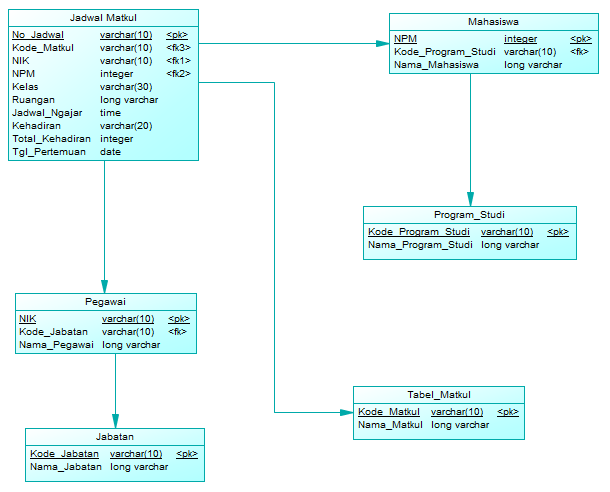
\includegraphics[width=10cm]{PDM}
\end{center}
disini suatu tabel masternya "JADWAL" ialah suatu induk informasi dari semua table yang telah saling berelasi bersama dengannya. dan setiap primary key yang bertamu akan menjadi foreignkey. 
di fase ini sudah menjadi Physical data yang benar sudak di check model dan sudah tidak memiliki lagi kesalahan seharusnya. terlihaf sangat beda dengan CDM. PDM ini sudak lebih terstruktur dan rapih menunjukkan relasinya.
\end{document}\textsl{•}
\end{document}
